\section{\MakeUppercase{Mathematical Formulation}}

\subsection{Mathematical Modeling in SIRENs}
\gls{siren} excel in tasks requiring the modeling of periodic and smooth phenomena, which are common in audio and video signals. The continuous nature of the function modeled by \gls{siren} makes them ideal for compressing these signals efficiently. The typical loss function used for training \gls{siren} in the context of compression is the \gls{mse}, which ensures the fidelity of the reconstructed signal:
\begin{equation}
    L = \frac{1}{N} \sum_{n=1}^N (\Phi(\mathbf{x}_n) - y_n)^2 
\end{equation}
Additionally, to capture temporal dynamics in video and audio, derivatives of the function are often included in the training objective:
\begin{equation}
    L = \frac{1}{N} \sum_{n=1}^N \left((\Phi(\mathbf{x}_n) - y_n)^2 + \lambda (\nabla\Phi(\mathbf{x}_n) - \nabla y_n)^2\right) 
\end{equation}
where, \( N \) is the total number of sampled points, \( \Phi \) is the SIREN model, \( \mathbf{x}_n \) are the input coordinates for the \(n\)-th data point, \( y_n \) are the actual output values at the \(n\)-th data point, \( \lambda \) is a regularization parameter, \( \nabla\Phi(\mathbf{x}_n) \) is the derivative of the \gls{siren} output with respect to the input at \( \mathbf{x}_n \), and \( \nabla y_n \) is the derivative of the true output values with respect to the input at \( \mathbf{x}_n \).


\subsection{Forward and Backward Propagation in SIREN Network}
\begin{figure}[H]
    \centering
    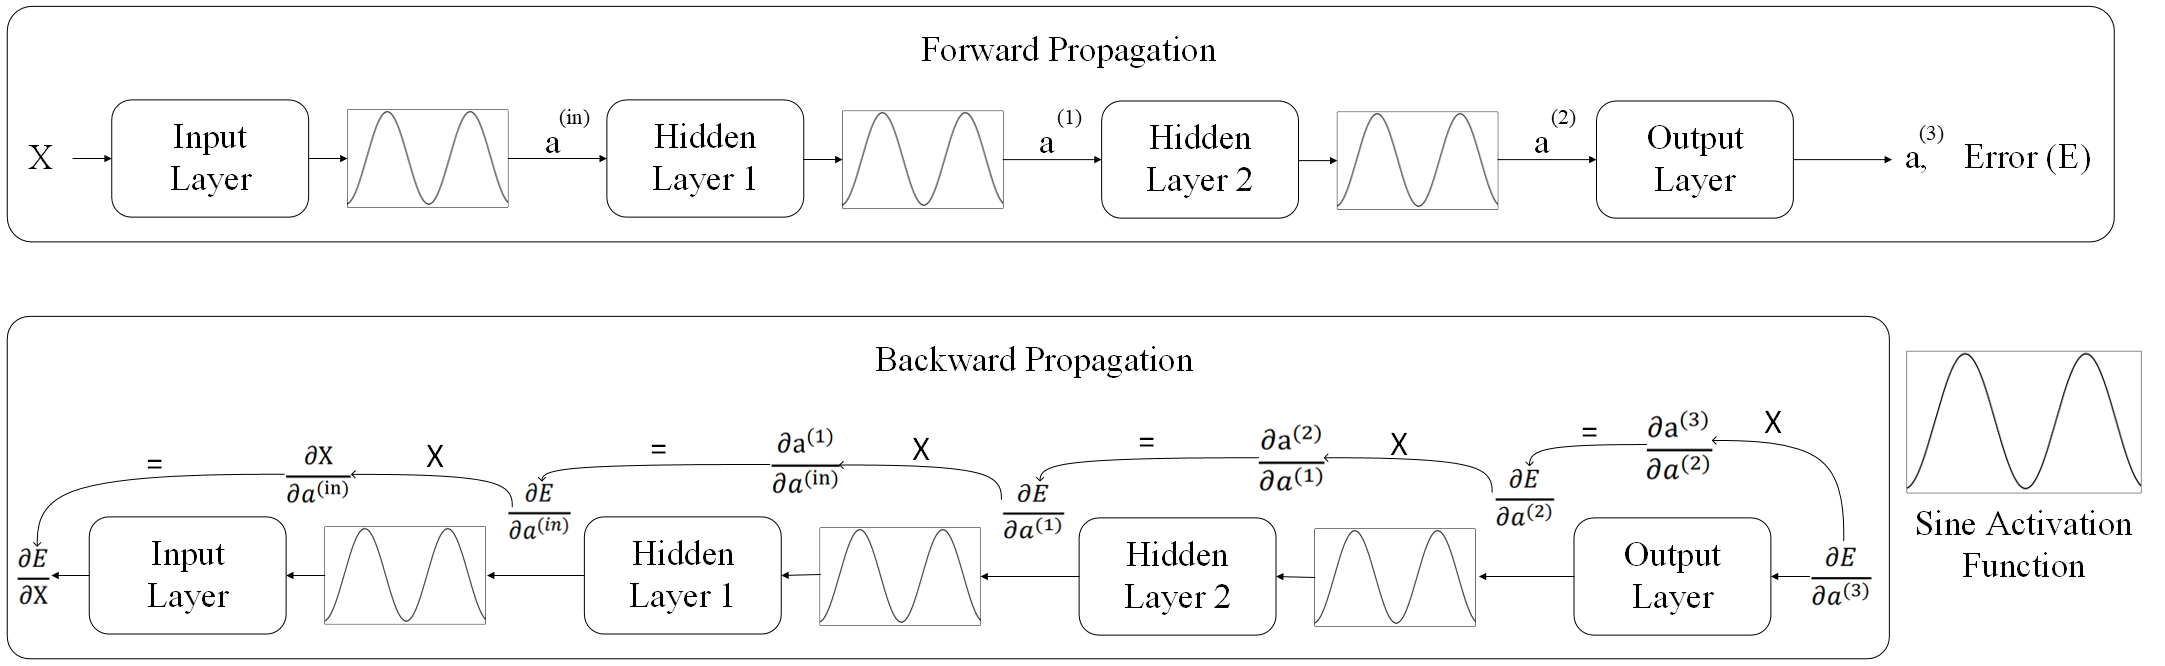
\includegraphics[width=\linewidth]{assets/Propagation concept figure Major Project.png}
    \caption{Forward and Backward Propagation in SIREN Network}
    \label{fig:propagation-diagram}
\end{figure}

The figure provides an illustration of the forward and backward propagation processes in a \gls{siren} neural network. In the forward propagation section, the input \( \mathbf{X} \) is passed through the input layer, then sine activation is applied, and then sequentially through hidden layers 1 (with sine activation) and hidden layer 2 (with sine activation), and finally through the output layer. The forward propagation process can be described by the equations:
\begin{equation}
    \mathbf{Z}^{(l)} = \mathbf{W}^{(l)T} \mathbf{a}^{(l-1)} + \mathbf{b}^{(l)}
\end{equation}
\begin{equation}
    \mathbf{a}^{(l)} = \sin(\mathbf{Z}^{(l)})
\end{equation}
where,
\begin{itemize}
    \item \( \mathbf{Z}^{(l)} \) is the linear combination of inputs at layer \( l \).
    \item \( \mathbf{W}^{(l)} \) represents the weights of the \( l \)-th layer.
    \item \( \mathbf{a}^{(l-1)} \) is the activation from the previous layer.
    \item \( \mathbf{b}^{(l)} \) represents the biases of the \( l \)-th layer.
    \item \( \mathbf{a}^{(l)} \) is the activation of the \( l \)-th layer after applying the sine function.
\end{itemize}

The error \( \mathbf{E} \) is calculated based on the difference between the predicted output \( \mathbf{a}^{(3)} \) and the actual output \( \mathbf{y}_i \). Specifically, we use the Mean Squared Error (MSE) loss function:
\begin{equation}
    \mathbf{E} = \frac{1}{2} \sum_{i=1}^{N} (\mathbf{a}^{(3)}_i - \mathbf{y}_i)^2
\end{equation}
where,
\begin{itemize}
    \item \( \mathbf{a}^{(3)}_i \) is the predicted output.
    \item \( \mathbf{y}_i \) is the actual output.
\end{itemize}

The backward propagation section shows the gradient calculation needed to update the network's weights. It starts with the error gradient \( \frac{\partial \mathbf{E}}{\partial \mathbf{a}^{(3)}} \) at the output layer and propagates backwards through hidden layers 2 and 1, and finally to the input layer. This involves computing the gradients \( \frac{\partial \mathbf{a}^{(3)}}{\partial \mathbf{a}^{(2)}} \), \( \frac{\partial \mathbf{a}^{(2)}}{\partial \mathbf{a}^{(1)}} \), and \( \frac{\partial \mathbf{a}^{(1)}}{\partial \mathbf{a}_{(in)}} \).

The weights and biases are updated as per the following equations:
\begin{equation}
    \mathbf{W}^{(l)} \leftarrow \mathbf{W}^{(l)} - \eta \frac{\partial \mathbf{E}}{\partial \mathbf{W}^{(l)}}  
\end{equation}
\begin{equation}
    \mathbf{b}^{(l)} \leftarrow \mathbf{b}^{(l)} - \eta \frac{\partial \mathbf{E}}{\partial \mathbf{b}^{(l)}}  
\end{equation}

where,
\begin{itemize}
    \item \( \mathbf{W}^{(l)} \) represents the weights of the \( l \)-th layer.
    \item \( \mathbf{b}^{(l)} \) represents the biases of the \( l \)-th layer.
    \item \( \eta \) is the learning rate.
    \item \( \frac{\partial \mathbf{E}}{\partial \mathbf{W}^{(l)}} \) is the gradient of the error with respect to the weights of the \( l \)-th layer.
    \item \( \frac{\partial \mathbf{E}}{\partial \mathbf{b}^{(l)}} \) is the gradient of the error with respect to the biases of the \( l \)-th layer.
\end{itemize}

The detailed forward and backward propagation equations and the gradients of error with respect to weight and bias matrices are provided in \autoref{app:forward-backward-eqn}.


\subsection{Quantization Modeling}
Quantization maps a floating-point weight \( w \) to a discrete integer \( w' \):


Then the dequantized value can be calculated as:
\begin{equation}
\text{dequantized value} = \text{quantized value} \cdot \text{scale}
\end{equation}



\begin{equation}
w' = \text{round}\Bigl(\frac{w}{s} + z\Bigr)
\label{eq:quantization_mapping}
\end{equation}
where:
\begin{itemize}
    \item \( w \in \mathbb{R} \) is the original floating-point weight.
    \item \( w' \in \mathbb{Z} \) is the quantized integer weight.
    \item \( s \in \mathbb{R}^+ \) is the scaling factor (step size).
    \item \( z \in \mathbb{R} \) is the zero-point, which may be a floating-point or integer value.
\end{itemize}

\subsubsection{Dequantization}
The dequantized value \( \hat{w} \) approximates the original floating-point value:
\begin{equation}
\hat{w} = s \cdot \bigl(w' - z\bigr)
\label{eq:dequantization}
\end{equation}

\subsubsection{Calculation of Scale and Zero-Point}
The scale \( s \) and zero-point \( z \) are determined based on 
the range of the floating-point weights \(\bigl[w_{\text{min}}, w_{\text{max}}\bigr]\) 
and the quantized range \(\bigl[q_{\text{min}}, q_{\text{max}}\bigr]\):
\begin{equation}
    s_{\text{asym}} = \frac{w_{\text{max}} - w_{\text{min}}}{2^n}
\label{eq:calc_scale_asym}
\end{equation}
\begin{equation}
    s_{\text{sym}} = \frac{\max\left(|w_{\text{min}}|, |w_{\text{max}}|\right)}{2^{n-1} - 1}
\label{eq:calc_scale_sym}
\end{equation}
\begin{equation}
    z_{\text{asym}} = q_{\text{min}} - \frac{w_{\text{min}}}{s_{\text{asym}}}
\label{eq:calc_zero_point_asym}
\end{equation}
\begin{equation}
    z_{\text{sym}} = 0
\label{eq:calc_zero_point_sym}
\end{equation}


\subsubsection{Quantization Error}
The error introduced by quantization is:
\begin{equation}
\epsilon = w - \hat{w}
\label{eq:quant_error}
\end{equation}
This is used in the calculation of \gls{sqnr} as explained in \autoref{subsubsec:SQNR}.

\subsection{Mathematical Formulation of the Arcsine Distribution}

We use the arcsine distribution in our analysis. The key mathematical properties of this distribution are outlined below, with detailed derivations provided in the appendix.

\subsubsection{Probability Density Function (PDF)}
The PDF of the arcsine distribution on the interval \((-1, 1)\) is given by:
\begin{equation}
f(x) = \frac{1}{\pi \sqrt{1-x^2}}
\end{equation}

\subsubsection{Cumulative Distribution Function (CDF)}
The cumulative distribution function (CDF), \( F(x) \), is defined as the integral of the probability density function (PDF) from the lower bound of the interval to \( x \):
\begin{equation}
F(x) = \int_{-1}^{x} f(t) \, dt
\end{equation}

\subsubsection{Mean}
The mean \(\mu\) of the distribution is calculated as follows:
\begin{equation}
\mu = \int_{-1}^{1} x f(x) \, dx = \int_{-1}^{1} x \cdot \frac{1}{\pi \sqrt{1-x^2}} \, dx
\end{equation}

\subsubsection{Variance}
The variance \(\sigma^2\) of the distribution is derived from the expected square and the square of the expected value:
\begin{equation}
\sigma^2 = \mathbf{E}[X^2] - (\mathbf{E}[X])^2
\end{equation}

These equations are fundamental to our project's analysis section and form the basis of our statistical analysis.

\pagebreak
